\documentclass[12pt,aspectratio=169]{beamer}
\usepackage[T1]{fontenc}
\usepackage{lmodern,amsmath,amssymb,booktabs,tikz,graphicx}
\usetikzlibrary{arrows.meta,positioning,calc}
\definecolor{Ink}{HTML}{17324D}
\definecolor{Teal}{HTML}{007F7A}
\definecolor{Muted}{HTML}{556574}
\definecolor{Paper}{HTML}{FAFAF7}
\definecolor{Rust}{HTML}{AD532E}
\definecolor{Gold}{HTML}{B38630}
\setbeamercolor{background canvas}{bg=Paper}
\setbeamercolor{normal text}{fg=Ink}
\setbeamercolor{frametitle}{fg=Ink}
\setbeamercolor{structure}{fg=Teal}
\setbeamercolor{alerted text}{fg=Rust}
\setbeamerfont{frametitle}{size=\LARGE,series=\bfseries}
\setbeamertemplate{navigation symbols}{}
\setbeamersize{text margin left=9mm,text margin right=9mm}
\setbeamertemplate{frametitle}{\par\vspace{2mm}\insertframetitle\par\vspace{1mm}{\color{Gold}\rule{14mm}{1pt}}}
\setbeamertemplate{footline}{\hspace{9mm}\scriptsize\color{Muted}\insertsectionhead\hfill\insertframenumber\hspace{9mm}\vspace{4mm}}
\hypersetup{colorlinks=true,urlcolor=Teal,linkcolor=Muted,pdfauthor={}}
\newcommand{\point}[1]{\par\vspace{3mm}{\large #1\par}}
\newcommand{\eqnote}[1]{\par\vspace{2mm}{\small\color{Muted}#1\par}}
\newcommand{\smalltext}[1]{\eqnote{#1}}
\newcommand{\insight}[1]{\par\vspace{2mm}{\color{Teal}\bfseries #1}\par}
\newcommand{\identity}{\text{\scriptsize accounting identity}}
\newcommand{\policy}{R^{\mathrm{policy}}}
\newcommand{\loanrate}{R^{\mathrm{loan}}}
\newcommand{\nominal}{R^{\mathrm{nom}}}
\newcommand{\realrate}{R^{\mathrm{real}}}
\newcommand{\neutral}{R^{\mathrm{neutral}}}
\newcommand{\spot}[1]{R^{\mathrm{spot}}(#1)}
\newcommand{\forward}[2]{R^{\mathrm{forward}}(#1,#2)}
\newcommand{\bondyield}{R^{\mathrm{bond}}}
\newcommand{\bondrate}[1]{R^{\mathrm{bond}}(#1)}
\AtBeginDocument{\setlength{\abovedisplayskip}{5pt}\setlength{\belowdisplayskip}{5pt}\setlength{\abovedisplayshortskip}{3pt}\setlength{\belowdisplayshortskip}{3pt}}

\hypersetup{pdftitle={Economics and Finance for Mathematicians: Open-economy policy and regimes}}
\begin{document}

% Slide 1: Open-economy policy and regimes

\begin{frame}[plain]
{\color{Teal}\large ECONOMICS AND FINANCE\quad /\quad 05}\par\vspace{9mm}{\Huge\bfseries Open-economy policy and regimes}\par\vspace{7mm}{\Large How does currency adjustment interact with demand and policy constraints?}
\end{frame}

% Slide 2: Today’s route

\begin{frame}{Today’s route}
\point{Trade prices and quantities determine the spending effect of FX.}\point{DD–AA connects output with asset-market equilibrium.}\point{Pegs, floating rates and the trilemma change the policy experiment.}
\end{frame}

% Slide 3: Trade prices and quantities
\section[Trade prices and quantities]{Trade prices and quantities}
\begin{frame}[plain]
{\color{Gold}\large LECTURE 5}\par\vspace{9mm}{\Huge\bfseries Trade prices and quantities}\par\vspace{7mm}{\Large Does a depreciation automatically improve the trade balance?}
\end{frame}

% Slide 4: Exporters and importers face different cash flows

\begin{frame}{Exporters and importers face different cash flows}
\begin{center}
\includegraphics[width=.93\textwidth,height=4.2cm,keepaspectratio]{assets/trade.png}\end{center}\eqnote{Invented trading economy. Imported inputs can be essential to domestic production.}
\end{frame}

% Slide 5: The real exchange rate and net exports

\begin{frame}{The real exchange rate and net exports}
\[q=\frac{EQ^{\rm foreign}}{Q^{\rm home}},\qquad NX=NX(q,Y,Y^{\rm foreign}).\]\point{A higher q makes home goods relatively cheaper.}\point{Higher home income can raise imports.}
\end{frame}

% Slide 6: A depreciation raises the local import bill first

\begin{frame}{A depreciation raises the local import bill first}
\begin{center}\begin{tabular}{@{}lll@{}}\toprule \textbf{Balanced trade initially} & \textbf{Before} & \textbf{Immediate effect}\\\midrule Real exchange rate q & 1.00 & 1.10\\[2mm]
Exports, fixed quantity and price & 100 & 100\\[2mm]
Import quantity, fixed & 100 & 100\\[2mm]
Home value of imports & 100 & 110\\[2mm]
Net exports & 0 & -10\\\bottomrule\end{tabular}\end{center}\eqnote{Producer-currency prices are fixed. Quantities have not adjusted.}
\end{frame}

% Slide 7: Quantities can later reverse the result

\begin{frame}{Quantities can later reverse the result}
\begin{center}\begin{tabular}{@{}ll@{}}\toprule \textbf{After the same depreciation} & \textbf{Value}\\\midrule Export volume rises 8\% & 108\\[2mm]
Import volume falls 6\% & 94\\[2mm]
Import value: 1.10 × 94 & 103.40\\[2mm]
Net exports: 108 - 103.40 & +4.60\\\bottomrule\end{tabular}\end{center}\eqnote{Invented quantity responses, after enough time to adjust.}
\end{frame}

% Slide 8: Marshall–Lerner gives a local condition

\begin{frame}{Marshall–Lerner gives a local condition}
\[\epsilon_X+\epsilon_M>1.\]\point{$\epsilon_X$: export-volume elasticity to real depreciation.}\point{$\epsilon_M$: absolute import-volume elasticity.}\eqnote{Balanced starting trade and fixed producer prices in the simplest derivation.}
\end{frame}

% Slide 9: The J-curve is a timing mechanism

\begin{frame}{The J-curve is a timing mechanism}
\begin{center}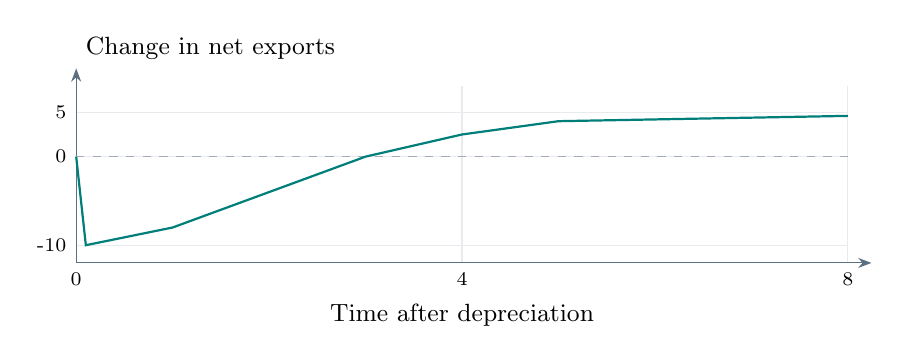
\begin{tikzpicture}[>=Stealth,every node/.style={font=\small}]
\draw[Ink!10] (0.0000,0.0000)--(0.0000,2.2500);\node[below,font=\scriptsize] at (0.0000,0.0000){0};
\draw[Ink!10] (4.9000,0.0000)--(4.9000,2.2500);\node[below,font=\scriptsize] at (4.9000,0.0000){4};
\draw[Ink!10] (9.8000,0.0000)--(9.8000,2.2500);\node[below,font=\scriptsize] at (9.8000,0.0000){8};
\draw[Ink!10] (0.0000,0.2250)--(9.8000,0.2250);\node[left,font=\scriptsize] at (0.0000,0.2250){-10};
\draw[Ink!10] (0.0000,1.3500)--(9.8000,1.3500);\node[left,font=\scriptsize] at (0.0000,1.3500){0};
\draw[Ink!10] (0.0000,1.9125)--(9.8000,1.9125);\node[left,font=\scriptsize] at (0.0000,1.9125){5};
\draw[->,Ink!70] (0,0)--(10.100000000000001,0);\draw[->,Ink!70] (0,0)--(0,2.47);
\node[below] at (4.9,-.40){Time after depreciation};\node[anchor=west] at (0,2.73){Change in net exports};
\draw[Ink!40,dashed] (0.0000,1.3500)--(9.8000,1.3500);
\draw[Teal,thick] plot coordinates {(0.0000,1.3500) (0.1225,0.2250) (1.2250,0.4500) (2.4500,0.9000) (3.6750,1.3500) (4.9000,1.6312) (6.1250,1.8000) (9.8000,1.8675)};
\end{tikzpicture}\end{center}\eqnote{Original hypothetical path: the import price effect precedes quantity adjustment.}
\end{frame}

% Slide 10: Invoice currency changes pass-through

\begin{frame}{Invoice currency changes pass-through}
\begin{center}\begin{tabular}{@{}lll@{}}\toprule \textbf{Euro exporter to a dollar buyer} & \textbf{Initial} & \textbf{After euro depreciation}\\\midrule USD per EUR & 1.10 & 1.00\\[2mm]
EUR invoice: EUR 100 in USD & 110 & 100\\[2mm]
USD invoice: USD 110 in USD & 110 & 110\\\bottomrule\end{tabular}\end{center}\eqnote{Same exchange-rate move. Different invoice contracts. Hypothetical prices.}
\end{frame}

% Slide 11: The dollar can matter in third-country trade

\begin{frame}{The dollar can matter in third-country trade}
\point{A UK importer buys from Korea at an invoice price of USD 100.}\point{GBP per USD rises from 0.80 to 0.88.}\point{The sterling bill rises from GBP 80 to GBP 88.}
\end{frame}

% Slide 12: The DD schedule
\section[The DD schedule]{The DD schedule}
\begin{frame}[plain]
{\color{Gold}\large LECTURE 5}\par\vspace{9mm}{\Huge\bfseries The DD schedule}\par\vspace{7mm}{\Large Which output and exchange-rate pairs balance the goods market?}
\end{frame}

% Slide 13: A short-run open-economy model

\begin{frame}{A short-run open-economy model}
\[Y=C(Y-T)+I+G+NX(q,Y,Y^{\rm foreign}).\]\point{Goods prices, foreign conditions and expected future FX are fixed.}\point{For this experiment, investment I is fixed too.}
\end{frame}

% Slide 14: A numerical demand equation

\begin{frame}{A numerical demand equation}
\[D=40+0.5Y+10E.\]\point{$D$: planned spending on home output.}\point{A higher E raises demand at each output level.}\point{Only half of extra output returns as extra planned spending.}
\end{frame}

% Slide 15: Goods-market equilibrium gives DD

\begin{frame}{Goods-market equilibrium gives DD}
\[Y=D\quad\Rightarrow\quad Y=80+20E.\]\point{A weaker currency raises demand and equilibrium output.}\point{DD slopes upward with Y horizontal and E vertical.}
\end{frame}

% Slide 16: DD as a graph

\begin{frame}{DD as a graph}
\begin{center}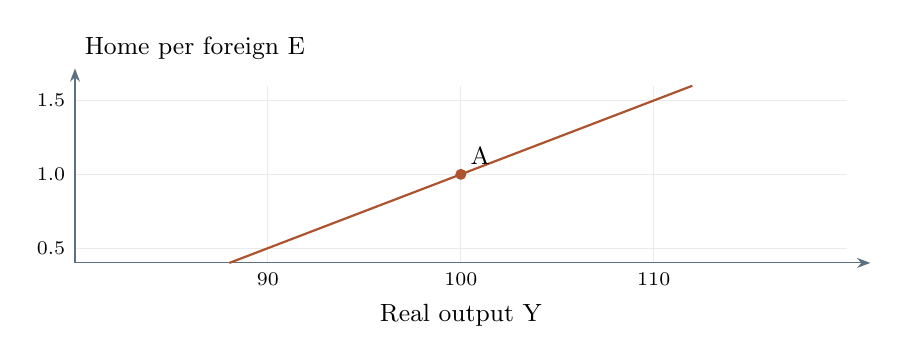
\begin{tikzpicture}[>=Stealth,every node/.style={font=\small}]
\draw[Ink!10] (2.4500,0.0000)--(2.4500,2.2500);\node[below,font=\scriptsize] at (2.4500,0.0000){90};
\draw[Ink!10] (4.9000,0.0000)--(4.9000,2.2500);\node[below,font=\scriptsize] at (4.9000,0.0000){100};
\draw[Ink!10] (7.3500,0.0000)--(7.3500,2.2500);\node[below,font=\scriptsize] at (7.3500,0.0000){110};
\draw[Ink!10] (0.0000,0.1875)--(9.8000,0.1875);\node[left,font=\scriptsize] at (0.0000,0.1875){0.5};
\draw[Ink!10] (0.0000,1.1250)--(9.8000,1.1250);\node[left,font=\scriptsize] at (0.0000,1.1250){1.0};
\draw[Ink!10] (0.0000,2.0625)--(9.8000,2.0625);\node[left,font=\scriptsize] at (0.0000,2.0625){1.5};
\draw[->,Ink!70] (0,0)--(10.100000000000001,0);\draw[->,Ink!70] (0,0)--(0,2.47);
\node[below] at (4.9,-.40){Real output Y};\node[anchor=west] at (0,2.73){Home per foreign E};
\draw[Rust,thick] plot coordinates {(1.9600,0.0000) (7.8400,2.2500)};
\fill[Rust] (4.9000,1.1250) circle (2pt);\node[above right] at (4.9000,1.1250){A};
\end{tikzpicture}\end{center}\eqnote{Original numerical goods-market equilibrium: Y = 80 + 20E.}
\end{frame}

% Slide 17: The AA schedule
\section[The AA schedule]{The AA schedule}
\begin{frame}[plain]
{\color{Gold}\large LECTURE 5}\par\vspace{9mm}{\Huge\bfseries The AA schedule}\par\vspace{7mm}{\Large What second relationship pins down output and the currency?}
\end{frame}

% Slide 18: Money demand and FX pricing together

\begin{frame}{Money demand and FX pricing together}
\[M/Q=L(Y,R^{\rm home}).\]\[R^{\rm home}\approx R^{\rm foreign}+\mathbb E_t\Delta\ln E.\]\point{Higher Y raises money demand and the home rate.}\point{At fixed expected future FX, that supports home appreciation.}
\end{frame}

% Slide 19: AA slopes downward

\begin{frame}{AA slopes downward}
\begin{center}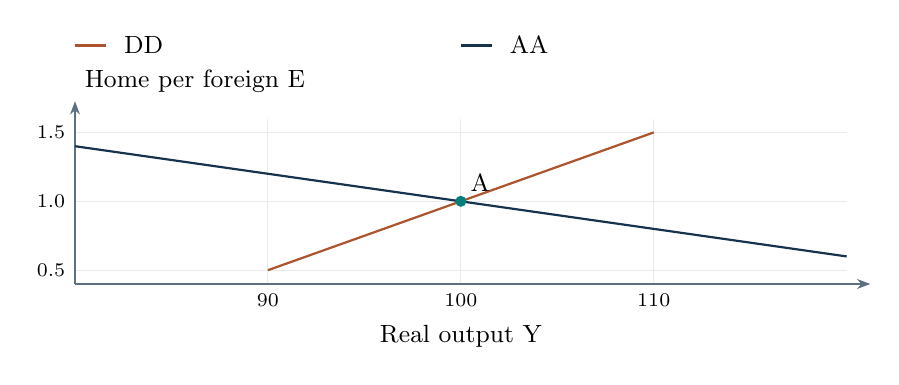
\begin{tikzpicture}[>=Stealth,every node/.style={font=\small}]
\draw[Ink!10] (2.4500,0.0000)--(2.4500,2.1000);\node[below,font=\scriptsize] at (2.4500,0.0000){90};
\draw[Ink!10] (4.9000,0.0000)--(4.9000,2.1000);\node[below,font=\scriptsize] at (4.9000,0.0000){100};
\draw[Ink!10] (7.3500,0.0000)--(7.3500,2.1000);\node[below,font=\scriptsize] at (7.3500,0.0000){110};
\draw[Ink!10] (0.0000,0.1750)--(9.8000,0.1750);\node[left,font=\scriptsize] at (0.0000,0.1750){0.5};
\draw[Ink!10] (0.0000,1.0500)--(9.8000,1.0500);\node[left,font=\scriptsize] at (0.0000,1.0500){1.0};
\draw[Ink!10] (0.0000,1.9250)--(9.8000,1.9250);\node[left,font=\scriptsize] at (0.0000,1.9250){1.5};
\draw[->,Ink!70] (0,0)--(10.100000000000001,0);\draw[->,Ink!70] (0,0)--(0,2.3200000000000003);
\node[below] at (4.9,-.40){Real output Y};\node[anchor=west] at (0,2.58){Home per foreign E};
\draw[Rust,thick] plot coordinates {(2.4500,0.1750) (7.3500,1.9250)};
\draw[Ink,thick] plot coordinates {(0.0000,1.7500) (9.8000,0.3500)};
\fill[Teal] (4.9000,1.0500) circle (2pt);\node[above right] at (4.9000,1.0500){A};
\draw[Rust,thick] (0.0,3.0300000000000002)--(0.4,3.0300000000000002);\node[anchor=west,font=\small] at (0.5,3.0300000000000002){DD};
\draw[Ink,thick] (4.9,3.0300000000000002)--(5.300000000000001,3.0300000000000002);\node[anchor=west,font=\small] at (5.4,3.0300000000000002){AA};
\end{tikzpicture}\end{center}\eqnote{The intersection A balances goods and asset markets. Original linear illustration.}
\end{frame}

% Slide 20: Temporary monetary expansion under a float

\begin{frame}{Temporary monetary expansion under a float}
\begin{center}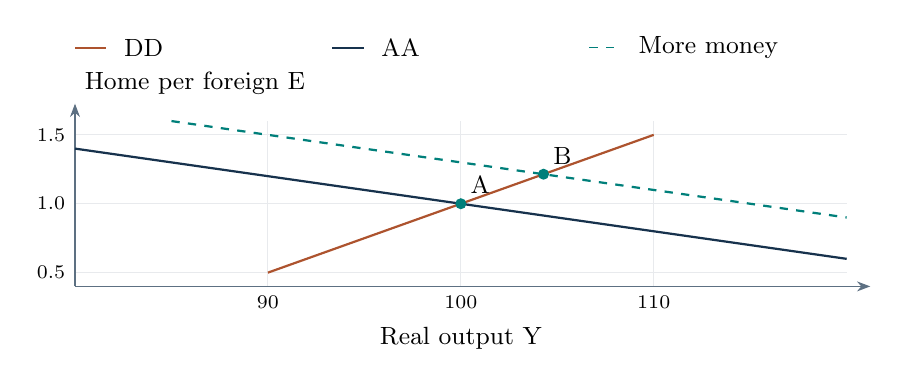
\begin{tikzpicture}[>=Stealth,every node/.style={font=\small}]
\draw[Ink!10] (2.4500,0.0000)--(2.4500,2.1000);\node[below,font=\scriptsize] at (2.4500,0.0000){90};
\draw[Ink!10] (4.9000,0.0000)--(4.9000,2.1000);\node[below,font=\scriptsize] at (4.9000,0.0000){100};
\draw[Ink!10] (7.3500,0.0000)--(7.3500,2.1000);\node[below,font=\scriptsize] at (7.3500,0.0000){110};
\draw[Ink!10] (0.0000,0.1750)--(9.8000,0.1750);\node[left,font=\scriptsize] at (0.0000,0.1750){0.5};
\draw[Ink!10] (0.0000,1.0500)--(9.8000,1.0500);\node[left,font=\scriptsize] at (0.0000,1.0500){1.0};
\draw[Ink!10] (0.0000,1.9250)--(9.8000,1.9250);\node[left,font=\scriptsize] at (0.0000,1.9250){1.5};
\draw[->,Ink!70] (0,0)--(10.100000000000001,0);\draw[->,Ink!70] (0,0)--(0,2.3200000000000003);
\node[below] at (4.9,-.40){Real output Y};\node[anchor=west] at (0,2.58){Home per foreign E};
\draw[Rust,thick] plot coordinates {(2.4500,0.1750) (7.3500,1.9250)};
\draw[Ink,thick] plot coordinates {(0.0000,1.7500) (9.8000,0.3500)};
\draw[Teal,dashed,thick] plot coordinates {(1.2250,2.1000) (9.8000,0.8750)};
\fill[Teal] (4.9000,1.0500) circle (2pt);\node[above right] at (4.9000,1.0500){A};
\fill[Teal] (5.9500,1.4250) circle (2pt);\node[above right] at (5.9500,1.4250){B};
\draw[Rust,thick] (0.0,3.0300000000000002)--(0.4,3.0300000000000002);\node[anchor=west,font=\small] at (0.5,3.0300000000000002){DD};
\draw[Ink,thick] (3.266666666666667,3.0300000000000002)--(3.666666666666667,3.0300000000000002);\node[anchor=west,font=\small] at (3.766666666666667,3.0300000000000002){AA};
\draw[Teal,dashed] (6.533333333333334,3.0300000000000002)--(6.9333333333333345,3.0300000000000002);\node[anchor=west,font=\small] at (7.033333333333334,3.0300000000000002){More money};
\end{tikzpicture}\end{center}\eqnote{AA shifts up. In this model output rises and the home currency depreciates.}
\end{frame}

% Slide 21: Temporary fiscal expansion under a float

\begin{frame}{Temporary fiscal expansion under a float}
\begin{center}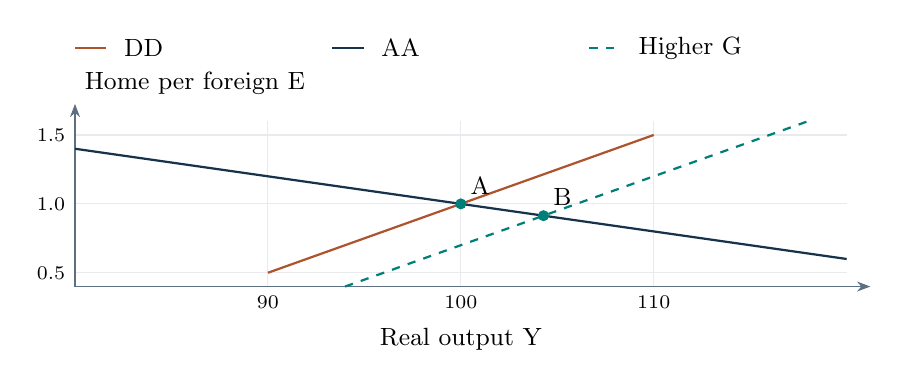
\begin{tikzpicture}[>=Stealth,every node/.style={font=\small}]
\draw[Ink!10] (2.4500,0.0000)--(2.4500,2.1000);\node[below,font=\scriptsize] at (2.4500,0.0000){90};
\draw[Ink!10] (4.9000,0.0000)--(4.9000,2.1000);\node[below,font=\scriptsize] at (4.9000,0.0000){100};
\draw[Ink!10] (7.3500,0.0000)--(7.3500,2.1000);\node[below,font=\scriptsize] at (7.3500,0.0000){110};
\draw[Ink!10] (0.0000,0.1750)--(9.8000,0.1750);\node[left,font=\scriptsize] at (0.0000,0.1750){0.5};
\draw[Ink!10] (0.0000,1.0500)--(9.8000,1.0500);\node[left,font=\scriptsize] at (0.0000,1.0500){1.0};
\draw[Ink!10] (0.0000,1.9250)--(9.8000,1.9250);\node[left,font=\scriptsize] at (0.0000,1.9250){1.5};
\draw[->,Ink!70] (0,0)--(10.100000000000001,0);\draw[->,Ink!70] (0,0)--(0,2.3200000000000003);
\node[below] at (4.9,-.40){Real output Y};\node[anchor=west] at (0,2.58){Home per foreign E};
\draw[Rust,thick] plot coordinates {(2.4500,0.1750) (7.3500,1.9250)};
\draw[Ink,thick] plot coordinates {(0.0000,1.7500) (9.8000,0.3500)};
\draw[Teal,dashed,thick] plot coordinates {(3.4300,0.0000) (9.3100,2.1000)};
\fill[Teal] (4.9000,1.0500) circle (2pt);\node[above right] at (4.9000,1.0500){A};
\fill[Teal] (5.9500,0.9000) circle (2pt);\node[above right] at (5.9500,0.9000){B};
\draw[Rust,thick] (0.0,3.0300000000000002)--(0.4,3.0300000000000002);\node[anchor=west,font=\small] at (0.5,3.0300000000000002){DD};
\draw[Ink,thick] (3.266666666666667,3.0300000000000002)--(3.666666666666667,3.0300000000000002);\node[anchor=west,font=\small] at (3.766666666666667,3.0300000000000002){AA};
\draw[Teal,dashed] (6.533333333333334,3.0300000000000002)--(6.9333333333333345,3.0300000000000002);\node[anchor=west,font=\small] at (7.033333333333334,3.0300000000000002){Higher G};
\end{tikzpicture}\end{center}\eqnote{DD shifts right. Output rises, while currency appreciation offsets some demand.}
\end{frame}

% Slide 22: A fiscal expansion need not improve net exports

\begin{frame}{A fiscal expansion need not improve net exports}
\point{Government demand rises directly.}\point{Higher income can increase imports.}\point{Appreciation can reduce expenditure switching toward home goods.}
\end{frame}

% Slide 23: At the lower bound, expectations still matter

\begin{frame}{At the lower bound, expectations still matter}
\point{Cash limits how far nominal rates can be pushed below zero.}\point{Extra reserves may have little effect on the current short rate.}\point{Credible changes in future policy can still affect real rates and FX.}
\end{frame}

% Slide 24: Pegs and interventions
\section[Pegs and interventions]{Pegs and interventions}
\begin{frame}[plain]
{\color{Gold}\large LECTURE 5}\par\vspace{9mm}{\Huge\bfseries Pegs and interventions}\par\vspace{7mm}{\Large What changes when the central bank promises a fixed currency price?}
\end{frame}

% Slide 25: The promise behind a peg

\begin{frame}{The promise behind a peg}
\point{The central bank stands ready to exchange currencies at the peg.}\point{It must supply foreign reserves when investors want to exit.}\point{The promise constrains monetary policy when capital moves freely.}
\end{frame}

% Slide 26: Defending a peg changes the balance sheet

\begin{frame}{Defending a peg changes the balance sheet}
\begin{center}\begin{tabular}{@{}lll@{}}\toprule \textbf{Central bank transaction} & \textbf{Assets} & \textbf{Liabilities}\\\midrule Sell 10 of foreign reserves & Foreign assets -10 & \\[2mm]
Receive home reserve balances &  & Bank reserves -10\\\bottomrule\end{tabular}\end{center}\point{An unsterilised sale drains domestic liquidity.}
\end{frame}

% Slide 27: Sterilisation offsets the liquidity effect

\begin{frame}{Sterilisation offsets the liquidity effect}
\begin{center}\begin{tabular}{@{}lll@{}}\toprule \textbf{Second transaction} & \textbf{Assets} & \textbf{Liabilities}\\\midrule Buy 10 of domestic bonds & Domestic assets +10 & Bank reserves +10\\\bottomrule\end{tabular}\end{center}\point{Total monetary liabilities return to their initial size.}\point{The asset portfolio now contains fewer foreign and more domestic assets.}
\end{frame}

% Slide 28: A fixed peg removes one degree of freedom

\begin{frame}{A fixed peg removes one degree of freedom}
\begin{center}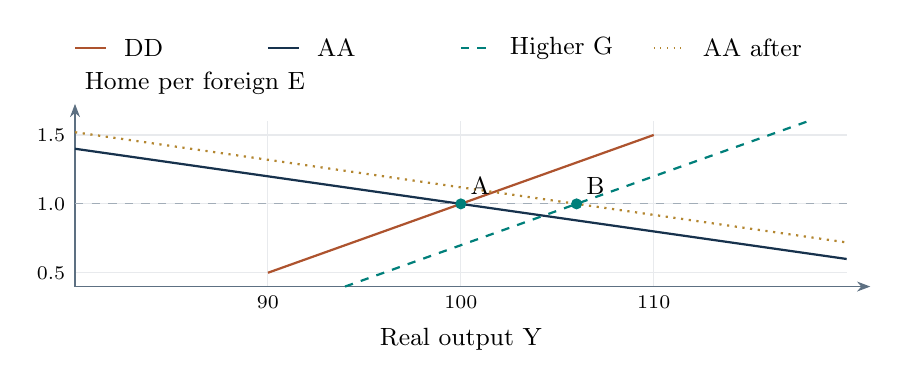
\begin{tikzpicture}[>=Stealth,every node/.style={font=\small}]
\draw[Ink!10] (2.4500,0.0000)--(2.4500,2.1000);\node[below,font=\scriptsize] at (2.4500,0.0000){90};
\draw[Ink!10] (4.9000,0.0000)--(4.9000,2.1000);\node[below,font=\scriptsize] at (4.9000,0.0000){100};
\draw[Ink!10] (7.3500,0.0000)--(7.3500,2.1000);\node[below,font=\scriptsize] at (7.3500,0.0000){110};
\draw[Ink!10] (0.0000,0.1750)--(9.8000,0.1750);\node[left,font=\scriptsize] at (0.0000,0.1750){0.5};
\draw[Ink!10] (0.0000,1.0500)--(9.8000,1.0500);\node[left,font=\scriptsize] at (0.0000,1.0500){1.0};
\draw[Ink!10] (0.0000,1.9250)--(9.8000,1.9250);\node[left,font=\scriptsize] at (0.0000,1.9250){1.5};
\draw[->,Ink!70] (0,0)--(10.100000000000001,0);\draw[->,Ink!70] (0,0)--(0,2.3200000000000003);
\node[below] at (4.9,-.40){Real output Y};\node[anchor=west] at (0,2.58){Home per foreign E};
\draw[Ink!40,dashed] (0.0000,1.0500)--(9.8000,1.0500);
\draw[Rust,thick] plot coordinates {(2.4500,0.1750) (7.3500,1.9250)};
\draw[Ink,thick] plot coordinates {(0.0000,1.7500) (9.8000,0.3500)};
\draw[Teal,dashed,thick] plot coordinates {(3.4300,0.0000) (9.3100,2.1000)};
\draw[Gold,dotted,thick] plot coordinates {(0.0000,1.9600) (9.8000,0.5600)};
\fill[Teal] (4.9000,1.0500) circle (2pt);\node[above right] at (4.9000,1.0500){A};
\fill[Teal] (6.3700,1.0500) circle (2pt);\node[above right] at (6.3700,1.0500){B};
\draw[Rust,thick] (0.0,3.0300000000000002)--(0.4,3.0300000000000002);\node[anchor=west,font=\small] at (0.5,3.0300000000000002){DD};
\draw[Ink,thick] (2.45,3.0300000000000002)--(2.85,3.0300000000000002);\node[anchor=west,font=\small] at (2.95,3.0300000000000002){AA};
\draw[Teal,dashed] (4.9,3.0300000000000002)--(5.300000000000001,3.0300000000000002);\node[anchor=west,font=\small] at (5.4,3.0300000000000002){Higher G};
\draw[Gold,dotted] (7.3500000000000005,3.0300000000000002)--(7.750000000000001,3.0300000000000002);\node[anchor=west,font=\small] at (7.8500000000000005,3.0300000000000002){AA after};
\end{tikzpicture}\end{center}\eqnote{At E = 1, higher G raises output from 100 to 106 if monetary policy accommodates.}
\end{frame}

% Slide 29: Independent monetary expansion conflicts with the peg

\begin{frame}{Independent monetary expansion conflicts with the peg}
\point{A rate cut creates pressure for home-currency depreciation.}\point{Defending the peg withdraws liquidity or reverses the rate cut.}\point{With an unchanged credible peg, the independent impulse cannot persist.}
\end{frame}

% Slide 30: The monetary trilemma

\begin{frame}{The monetary trilemma}
\begin{center}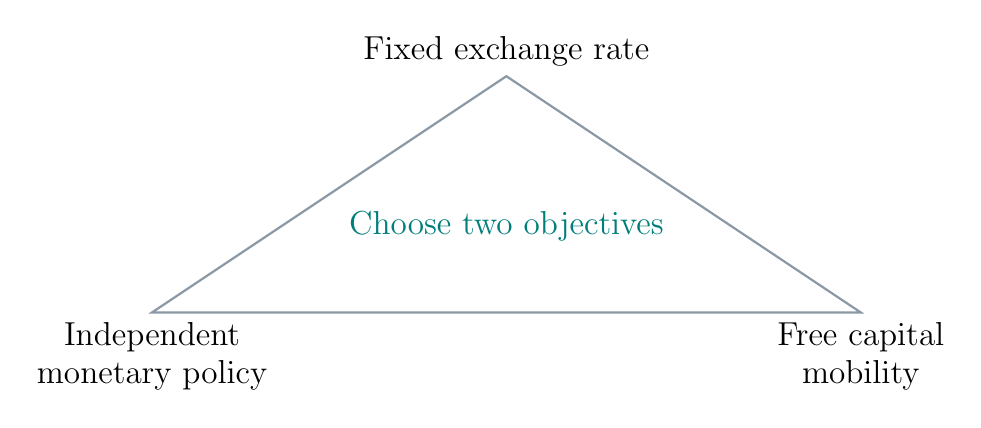
\begin{tikzpicture}[every node/.style={font=\large,align=center}]\draw[Ink!50,thick](0,0)--(9,0)--(4.5,3)--cycle;\node[above]at(4.5,3){Fixed exchange rate};\node[below]at(0,0){Independent\\monetary policy};\node[below]at(9,0){Free capital\\mobility};\node[Teal]at(4.5,1.1){Choose two objectives};\end{tikzpicture}\end{center}
\end{frame}

% Slide 31: Gold and the international system
\section[Gold and the international system]{Gold and the international system}
\begin{frame}[plain]
{\color{Gold}\large LECTURE 5}\par\vspace{9mm}{\Huge\bfseries Gold and the international system}\par\vspace{7mm}{\Large What does a monetary anchor buy, and what adjustment does it impose?}
\end{frame}

% Slide 32: Gold convertibility

\begin{frame}{Gold convertibility}
\begin{center}
\includegraphics[width=.93\textwidth,height=4.2cm,keepaspectratio]{assets/gold.png}\end{center}\eqnote{Illustration of redemption, not a historical photograph or certificate.}
\end{frame}

% Slide 33: Gold fixes a currency relationship

\begin{frame}{Gold fixes a currency relationship}
\[1\text{ home unit}=a\text{ grams},\qquad1\text{ foreign unit}=b\text{ grams}.\]\[E=\frac{b}{a}\quad\text{home units per foreign unit}.\]\eqnote{Transport, insurance and conversion costs create a band around parity.}
\end{frame}

% Slide 34: Deflation makes a fixed nominal rate tighter

\begin{frame}{Deflation makes a fixed nominal rate tighter}
\[\nominal=0\%,\quad\mathbb E\pi=-5\%\quad\Rightarrow\quad\realrate\approx5\%.\]\point{Falling expected prices can raise the real cost of borrowing.}\point{A monetary anchor can constrain the response.}
\end{frame}

% Slide 35: Three monetary arrangements

\begin{frame}{Three monetary arrangements}
\begin{center}\begin{tabular}{@{}p{.23\textwidth}p{.31\textwidth}p{.39\textwidth}@{}}\toprule \textbf{Arrangement} & \textbf{Anchor} & \textbf{Adjustment problem}\\\midrule Gold standard & Gold convertibility & Domestic demand may bear the strain\\[2mm]
Bretton Woods & Dollar pegs and dollar-gold link & Reserve demand versus convertibility\\[2mm]
Floating fiat currencies & Domestic policy frameworks & FX absorbs shocks, can also amplify them\\\bottomrule\end{tabular}\end{center}
\end{frame}

% Slide 36: Triffin’s dilemma

\begin{frame}{Triffin’s dilemma}
\point{Global demand for dollar reserves requires dollar liabilities.}\point{More claims relative to gold can weaken confidence in convertibility.}\point{Providing liquidity and preserving a fixed gold promise can conflict.}
\end{frame}

% Slide 37: Counterfactual exercise: who can ease?

\begin{frame}{Counterfactual exercise: who can ease?}
\begin{center}\begin{tabular}{@{}lll@{}}\toprule \textbf{Economy} & \textbf{Regime} & \textbf{Can cut independently?}\\\midrule A & Float, mobile capital & ?\\[2mm]
B & Credible peg, mobile capital & ?\\[2mm]
C & Peg, effective capital controls & ?\\\bottomrule\end{tabular}\end{center}\eqnote{Assume the foreign policy rate stays fixed and no devaluation is expected.}
\end{frame}

% Slide 38: Further reading
\section[Reading]{Reading}
\begin{frame}{Further reading}
\point{Dmitriy Sergeyev, Bocconi 30054 course materials.}\point{Krugman, Obstfeld \& Melitz, \emph{International Economics}.}\point{Source links and worked answers accompany each slide in the notes.}
\end{frame}
\end{document}
